% Created by tikzDevice version 0.12.4 on 2023-06-03 15:47:54
% !TEX encoding = UTF-8 Unicode
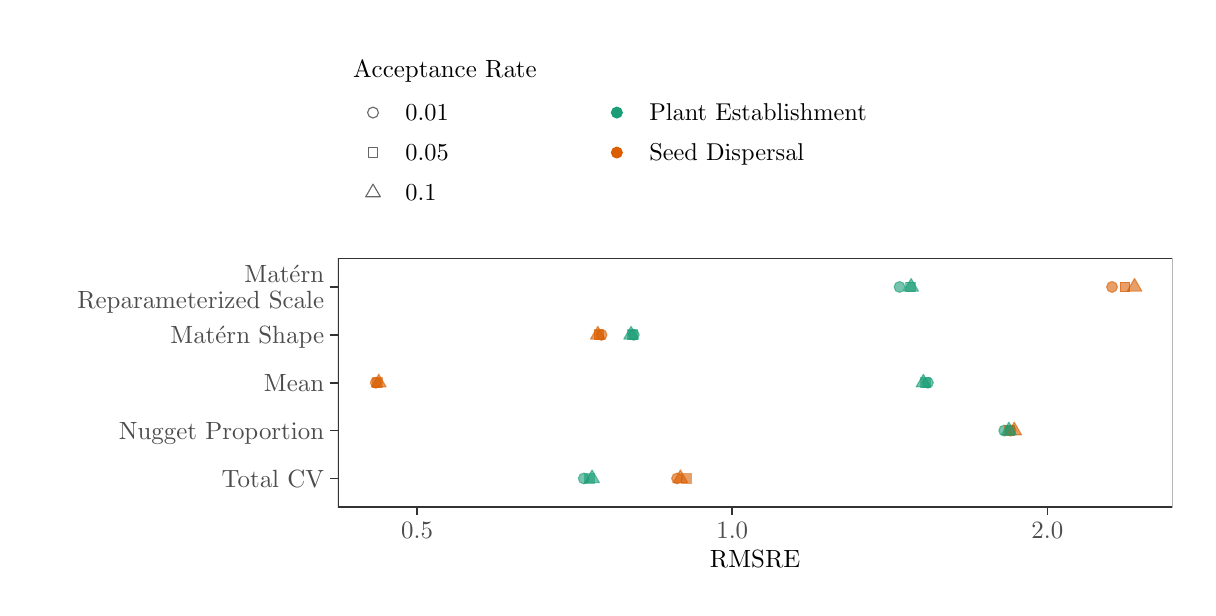
\begin{tikzpicture}[x=1pt,y=1pt]
\definecolor{fillColor}{RGB}{255,255,255}
\path[use as bounding box,fill=fillColor,fill opacity=0.00] (0,0) rectangle (419.17,202.36);
\begin{scope}
\path[clip] (  0.00,  0.00) rectangle (419.17,202.36);
\definecolor{drawColor}{RGB}{255,255,255}
\definecolor{fillColor}{RGB}{255,255,255}

\path[draw=drawColor,line width= 0.6pt,line join=round,line cap=round,fill=fillColor] (  0.00,  0.00) rectangle (419.17,202.36);
\end{scope}
\begin{scope}
\path[clip] (112.07, 29.10) rectangle (413.67,119.05);
\definecolor{fillColor}{RGB}{255,255,255}

\path[fill=fillColor] (112.07, 29.10) rectangle (413.67,119.05);
\definecolor{drawColor}{RGB}{217,95,2}
\definecolor{fillColor}{RGB}{217,95,2}

\path[draw=drawColor,draw opacity=0.60,line width= 0.4pt,line join=round,line cap=round,fill=fillColor,fill opacity=0.60] (391.83,108.67) circle (  1.96);

\path[draw=drawColor,draw opacity=0.60,line width= 0.4pt,line join=round,line cap=round,fill=fillColor,fill opacity=0.60] (207.37, 91.37) circle (  1.96);

\path[draw=drawColor,draw opacity=0.60,line width= 0.4pt,line join=round,line cap=round,fill=fillColor,fill opacity=0.60] (234.65, 39.47) circle (  1.96);

\path[draw=drawColor,draw opacity=0.60,line width= 0.4pt,line join=round,line cap=round,fill=fillColor,fill opacity=0.60] (355.21, 56.77) circle (  1.96);

\path[draw=drawColor,draw opacity=0.60,line width= 0.4pt,line join=round,line cap=round,fill=fillColor,fill opacity=0.60] (125.78, 74.07) circle (  1.96);
\definecolor{drawColor}{RGB}{27,158,119}
\definecolor{fillColor}{RGB}{27,158,119}

\path[draw=drawColor,draw opacity=0.60,line width= 0.4pt,line join=round,line cap=round,fill=fillColor,fill opacity=0.60] (315.05,108.67) circle (  1.96);

\path[draw=drawColor,draw opacity=0.60,line width= 0.4pt,line join=round,line cap=round,fill=fillColor,fill opacity=0.60] (219.02, 91.37) circle (  1.96);

\path[draw=drawColor,draw opacity=0.60,line width= 0.4pt,line join=round,line cap=round,fill=fillColor,fill opacity=0.60] (200.94, 39.47) circle (  1.96);

\path[draw=drawColor,draw opacity=0.60,line width= 0.4pt,line join=round,line cap=round,fill=fillColor,fill opacity=0.60] (352.86, 56.77) circle (  1.96);

\path[draw=drawColor,draw opacity=0.60,line width= 0.4pt,line join=round,line cap=round,fill=fillColor,fill opacity=0.60] (325.28, 74.07) circle (  1.96);
\definecolor{drawColor}{RGB}{217,95,2}
\definecolor{fillColor}{RGB}{217,95,2}

\path[draw=drawColor,draw opacity=0.60,line width= 0.4pt,line join=round,line cap=round,fill=fillColor,fill opacity=0.60] (394.74,106.93) rectangle (398.21,110.41);

\path[draw=drawColor,draw opacity=0.60,line width= 0.4pt,line join=round,line cap=round,fill=fillColor,fill opacity=0.60] (204.74, 89.63) rectangle (208.22, 93.11);

\path[draw=drawColor,draw opacity=0.60,line width= 0.4pt,line join=round,line cap=round,fill=fillColor,fill opacity=0.60] (236.30, 37.74) rectangle (239.78, 41.21);

\path[draw=drawColor,draw opacity=0.60,line width= 0.4pt,line join=round,line cap=round,fill=fillColor,fill opacity=0.60] (353.02, 55.03) rectangle (356.50, 58.51);

\path[draw=drawColor,draw opacity=0.60,line width= 0.4pt,line join=round,line cap=round,fill=fillColor,fill opacity=0.60] (124.67, 72.33) rectangle (128.15, 75.81);
\definecolor{drawColor}{RGB}{27,158,119}
\definecolor{fillColor}{RGB}{27,158,119}

\path[draw=drawColor,draw opacity=0.60,line width= 0.4pt,line join=round,line cap=round,fill=fillColor,fill opacity=0.60] (317.22,106.93) rectangle (320.70,110.41);

\path[draw=drawColor,draw opacity=0.60,line width= 0.4pt,line join=round,line cap=round,fill=fillColor,fill opacity=0.60] (216.82, 89.63) rectangle (220.30, 93.11);

\path[draw=drawColor,draw opacity=0.60,line width= 0.4pt,line join=round,line cap=round,fill=fillColor,fill opacity=0.60] (201.33, 37.74) rectangle (204.81, 41.21);

\path[draw=drawColor,draw opacity=0.60,line width= 0.4pt,line join=round,line cap=round,fill=fillColor,fill opacity=0.60] (353.24, 55.03) rectangle (356.72, 58.51);

\path[draw=drawColor,draw opacity=0.60,line width= 0.4pt,line join=round,line cap=round,fill=fillColor,fill opacity=0.60] (322.73, 72.33) rectangle (326.20, 75.81);
\definecolor{drawColor}{RGB}{217,95,2}
\definecolor{fillColor}{RGB}{217,95,2}

\path[draw=drawColor,draw opacity=0.60,line width= 0.4pt,line join=round,line cap=round,fill=fillColor,fill opacity=0.60] (399.96,111.72) --
	(402.60,107.14) --
	(397.31,107.14) --
	cycle;

\path[draw=drawColor,draw opacity=0.60,line width= 0.4pt,line join=round,line cap=round,fill=fillColor,fill opacity=0.60] (206.02, 94.42) --
	(208.66, 89.84) --
	(203.37, 89.84) --
	cycle;

\path[draw=drawColor,draw opacity=0.60,line width= 0.4pt,line join=round,line cap=round,fill=fillColor,fill opacity=0.60] (235.87, 42.53) --
	(238.51, 37.95) --
	(233.23, 37.95) --
	cycle;

\path[draw=drawColor,draw opacity=0.60,line width= 0.4pt,line join=round,line cap=round,fill=fillColor,fill opacity=0.60] (356.49, 59.82) --
	(359.13, 55.25) --
	(353.84, 55.25) --
	cycle;

\path[draw=drawColor,draw opacity=0.60,line width= 0.4pt,line join=round,line cap=round,fill=fillColor,fill opacity=0.60] (126.87, 77.12) --
	(129.51, 72.55) --
	(124.22, 72.55) --
	cycle;
\definecolor{drawColor}{RGB}{27,158,119}
\definecolor{fillColor}{RGB}{27,158,119}

\path[draw=drawColor,draw opacity=0.60,line width= 0.4pt,line join=round,line cap=round,fill=fillColor,fill opacity=0.60] (319.24,111.72) --
	(321.88,107.14) --
	(316.59,107.14) --
	cycle;

\path[draw=drawColor,draw opacity=0.60,line width= 0.4pt,line join=round,line cap=round,fill=fillColor,fill opacity=0.60] (218.04, 94.42) --
	(220.68, 89.84) --
	(215.39, 89.84) --
	cycle;

\path[draw=drawColor,draw opacity=0.60,line width= 0.4pt,line join=round,line cap=round,fill=fillColor,fill opacity=0.60] (203.95, 42.53) --
	(206.60, 37.95) --
	(201.31, 37.95) --
	cycle;

\path[draw=drawColor,draw opacity=0.60,line width= 0.4pt,line join=round,line cap=round,fill=fillColor,fill opacity=0.60] (354.55, 59.82) --
	(357.19, 55.25) --
	(351.90, 55.25) --
	cycle;

\path[draw=drawColor,draw opacity=0.60,line width= 0.4pt,line join=round,line cap=round,fill=fillColor,fill opacity=0.60] (323.67, 77.12) --
	(326.31, 72.55) --
	(321.03, 72.55) --
	cycle;
\definecolor{drawColor}{gray}{0.20}

\path[draw=drawColor,line width= 0.6pt,line join=round,line cap=round] (112.07, 29.10) rectangle (413.67,119.05);
\end{scope}
\begin{scope}
\path[clip] (  0.00,  0.00) rectangle (419.17,202.36);
\definecolor{drawColor}{gray}{0.30}

\node[text=drawColor,anchor=base east,inner sep=0pt, outer sep=0pt, scale=  0.90] at (107.12, 36.38) {Total CV};

\node[text=drawColor,anchor=base east,inner sep=0pt, outer sep=0pt, scale=  0.90] at (107.12, 53.67) {Nugget Proportion};

\node[text=drawColor,anchor=base east,inner sep=0pt, outer sep=0pt, scale=  0.90] at (107.12, 70.97) {Mean};

\node[text=drawColor,anchor=base east,inner sep=0pt, outer sep=0pt, scale=  0.90] at (107.12, 88.27) {Matérn Shape};

\node[text=drawColor,anchor=base east,inner sep=0pt, outer sep=0pt, scale=  0.90] at (107.12,110.43) {Matérn};

\node[text=drawColor,anchor=base east,inner sep=0pt, outer sep=0pt, scale=  0.90] at (107.12,100.71) {Reparameterized Scale};
\end{scope}
\begin{scope}
\path[clip] (  0.00,  0.00) rectangle (419.17,202.36);
\definecolor{drawColor}{gray}{0.20}

\path[draw=drawColor,line width= 0.6pt,line join=round] (109.32, 39.47) --
	(112.07, 39.47);

\path[draw=drawColor,line width= 0.6pt,line join=round] (109.32, 56.77) --
	(112.07, 56.77);

\path[draw=drawColor,line width= 0.6pt,line join=round] (109.32, 74.07) --
	(112.07, 74.07);

\path[draw=drawColor,line width= 0.6pt,line join=round] (109.32, 91.37) --
	(112.07, 91.37);

\path[draw=drawColor,line width= 0.6pt,line join=round] (109.32,108.67) --
	(112.07,108.67);
\end{scope}
\begin{scope}
\path[clip] (  0.00,  0.00) rectangle (419.17,202.36);
\definecolor{drawColor}{gray}{0.20}

\path[draw=drawColor,line width= 0.6pt,line join=round] (140.72, 26.35) --
	(140.72, 29.10);

\path[draw=drawColor,line width= 0.6pt,line join=round] (254.59, 26.35) --
	(254.59, 29.10);

\path[draw=drawColor,line width= 0.6pt,line join=round] (368.46, 26.35) --
	(368.46, 29.10);
\end{scope}
\begin{scope}
\path[clip] (  0.00,  0.00) rectangle (419.17,202.36);
\definecolor{drawColor}{gray}{0.30}

\node[text=drawColor,anchor=base,inner sep=0pt, outer sep=0pt, scale=  0.90] at (140.72, 17.95) {0.5};

\node[text=drawColor,anchor=base,inner sep=0pt, outer sep=0pt, scale=  0.90] at (254.59, 17.95) {1.0};

\node[text=drawColor,anchor=base,inner sep=0pt, outer sep=0pt, scale=  0.90] at (368.46, 17.95) {2.0};
\end{scope}
\begin{scope}
\path[clip] (  0.00,  0.00) rectangle (419.17,202.36);
\definecolor{drawColor}{RGB}{0,0,0}

\node[text=drawColor,anchor=base,inner sep=0pt, outer sep=0pt, scale=  0.90] at (262.87,  7.25) {RMSRE};
\end{scope}
\begin{scope}
\path[clip] (  0.00,  0.00) rectangle (419.17,202.36);
\definecolor{fillColor}{RGB}{255,255,255}

\path[fill=fillColor] (112.07,130.05) rectangle (189.18,196.86);
\end{scope}
\begin{scope}
\path[clip] (  0.00,  0.00) rectangle (419.17,202.36);
\definecolor{drawColor}{RGB}{0,0,0}

\node[text=drawColor,anchor=base west,inner sep=0pt, outer sep=0pt, scale=  0.90] at (117.57,184.28) {Acceptance Rate};
\end{scope}
\begin{scope}
\path[clip] (  0.00,  0.00) rectangle (419.17,202.36);
\definecolor{fillColor}{RGB}{255,255,255}

\path[fill=fillColor] (117.57,164.45) rectangle (132.02,178.91);
\end{scope}
\begin{scope}
\path[clip] (  0.00,  0.00) rectangle (419.17,202.36);
\definecolor{drawColor}{RGB}{0,0,0}

\path[draw=drawColor,draw opacity=0.60,line width= 0.4pt,line join=round,line cap=round] (124.79,171.68) circle (  1.96);
\end{scope}
\begin{scope}
\path[clip] (  0.00,  0.00) rectangle (419.17,202.36);
\definecolor{fillColor}{RGB}{255,255,255}

\path[fill=fillColor] (117.57,150.00) rectangle (132.02,164.45);
\end{scope}
\begin{scope}
\path[clip] (  0.00,  0.00) rectangle (419.17,202.36);
\definecolor{drawColor}{RGB}{0,0,0}

\path[draw=drawColor,draw opacity=0.60,line width= 0.4pt,line join=round,line cap=round] (123.06,155.49) rectangle (126.53,158.97);
\end{scope}
\begin{scope}
\path[clip] (  0.00,  0.00) rectangle (419.17,202.36);
\definecolor{fillColor}{RGB}{255,255,255}

\path[fill=fillColor] (117.57,135.55) rectangle (132.02,150.00);
\end{scope}
\begin{scope}
\path[clip] (  0.00,  0.00) rectangle (419.17,202.36);
\definecolor{drawColor}{RGB}{0,0,0}

\path[draw=drawColor,draw opacity=0.60,line width= 0.4pt,line join=round,line cap=round] (124.79,145.82) --
	(127.44,141.25) --
	(122.15,141.25) --
	cycle;
\end{scope}
\begin{scope}
\path[clip] (  0.00,  0.00) rectangle (419.17,202.36);
\definecolor{drawColor}{RGB}{0,0,0}

\node[text=drawColor,anchor=base west,inner sep=0pt, outer sep=0pt, scale=  0.88] at (136.52,168.65) {0.01};
\end{scope}
\begin{scope}
\path[clip] (  0.00,  0.00) rectangle (419.17,202.36);
\definecolor{drawColor}{RGB}{0,0,0}

\node[text=drawColor,anchor=base west,inner sep=0pt, outer sep=0pt, scale=  0.88] at (136.52,154.20) {0.05};
\end{scope}
\begin{scope}
\path[clip] (  0.00,  0.00) rectangle (419.17,202.36);
\definecolor{drawColor}{RGB}{0,0,0}

\node[text=drawColor,anchor=base west,inner sep=0pt, outer sep=0pt, scale=  0.88] at (136.52,139.74) {0.1};
\end{scope}
\begin{scope}
\path[clip] (  0.00,  0.00) rectangle (419.17,202.36);
\definecolor{fillColor}{RGB}{255,255,255}

\path[fill=fillColor] (200.18,144.50) rectangle (308.68,196.86);
\end{scope}
\begin{scope}
\path[clip] (  0.00,  0.00) rectangle (419.17,202.36);
\definecolor{fillColor}{RGB}{255,255,255}

\path[fill=fillColor] (205.68,164.45) rectangle (220.13,178.91);
\end{scope}
\begin{scope}
\path[clip] (  0.00,  0.00) rectangle (419.17,202.36);
\definecolor{drawColor}{RGB}{27,158,119}
\definecolor{fillColor}{RGB}{27,158,119}

\path[draw=drawColor,line width= 0.4pt,line join=round,line cap=round,fill=fillColor] (212.90,171.68) circle (  1.96);
\end{scope}
\begin{scope}
\path[clip] (  0.00,  0.00) rectangle (419.17,202.36);
\definecolor{fillColor}{RGB}{255,255,255}

\path[fill=fillColor] (205.68,150.00) rectangle (220.13,164.45);
\end{scope}
\begin{scope}
\path[clip] (  0.00,  0.00) rectangle (419.17,202.36);
\definecolor{drawColor}{RGB}{217,95,2}
\definecolor{fillColor}{RGB}{217,95,2}

\path[draw=drawColor,line width= 0.4pt,line join=round,line cap=round,fill=fillColor] (212.90,157.23) circle (  1.96);
\end{scope}
\begin{scope}
\path[clip] (  0.00,  0.00) rectangle (419.17,202.36);
\definecolor{drawColor}{RGB}{0,0,0}

\node[text=drawColor,anchor=base west,inner sep=0pt, outer sep=0pt, scale=  0.88] at (224.63,168.65) {Plant Establishment};
\end{scope}
\begin{scope}
\path[clip] (  0.00,  0.00) rectangle (419.17,202.36);
\definecolor{drawColor}{RGB}{0,0,0}

\node[text=drawColor,anchor=base west,inner sep=0pt, outer sep=0pt, scale=  0.88] at (224.63,154.20) {Seed Dispersal};
\end{scope}
\end{tikzpicture}
